Since $u(x,t)\to0$ (resp. 1) as $x\to\infty$ (resp. $-\infty$), we can approximate the traveling
wave given in (i) in $(-L,L)$ wehre $L$ is large enough so that the wave front does not reach the
boundary $x=L$, by imposing the boundary conditions

$$u(-L,t) = 1,\;\;u(L,t) = 0$$

and taking the initial value as $u(x,0)$. Design and implement a Chebyshev collocation method to
approximate the solution of the PDE and study the convergence of the approximate solution as $N$ is
increasing.\\

\begin{solution}\renewcommand{\qedsymbol}{}\ \\
    Since we are truncating the length of the domain, we set $L=50$. So, using the Chebyshev
    differentiation matrix, we can set up a linear system in $x$ and then do a time stepping process.
    For this, we use Euler time stepping. We also use $u(x,0)=0$ as our initial condition,
    and then $u(-50,t)=1$ and $u(50,t)=0$ as our boundary conditions. So, using the following code, we
    get the following plot.

    \begin{center}
        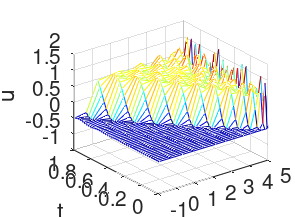
\includegraphics[scale=1]{problem2ii.PNG}
    \end{center}

\end{solution}

\newpage
\lstinputlisting{problem2ii.m}
\newpage